\chapter{Modeling and Controller Design for the TU/e \texorpdfstring{$1$}{1}-DoF System}
\label{chap:application}
In this chapter, the synthesis conditions of the previous chapter is applied to a $1$-DOF experimental setup. Different
uncertainty structures are considered and compared. 


\begin{figure}%
\centering
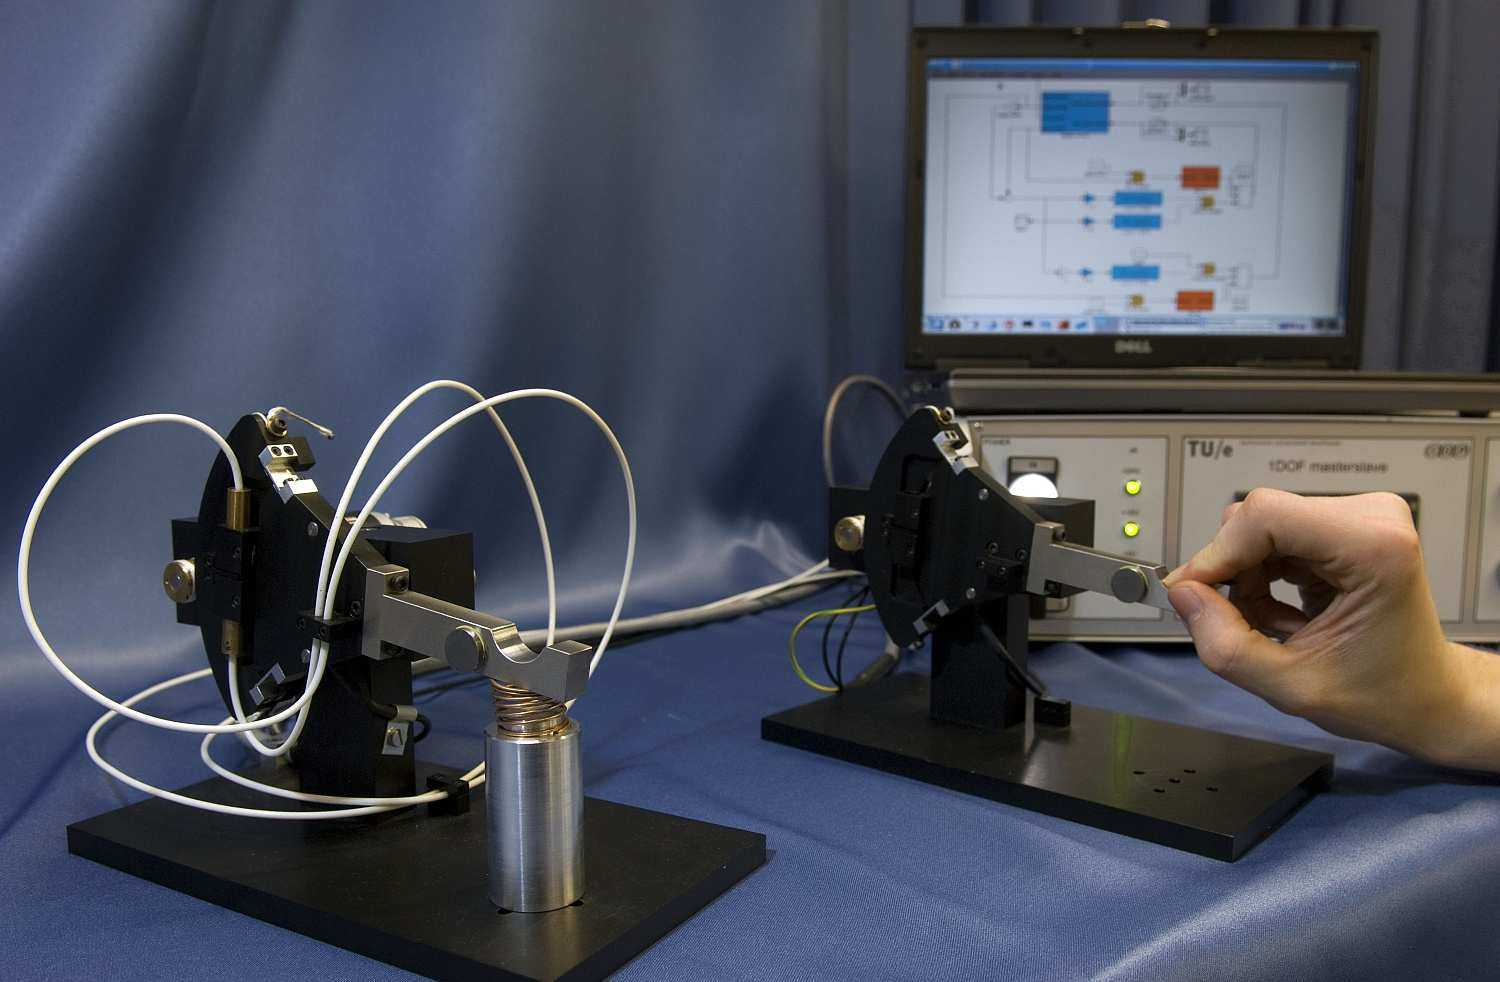
\includegraphics[width=0.6\columnwidth]{\impath/application/hendrix1dof}%
\caption[TU/e $1$-DoF Experimental Setup]{TU/e $1$-DoF Experimental Setup (Image is taken from \cite{hendrix})}%
\label{fig:app:onedof}%
\end{figure}

\section{The experimental setup}
At the Control Systems Technology department of Eindhoven University of Technology, a 1-Degree-of-Freedom prototype has been realized 
within the project of constructing a 5-DoF haptics local device for robotically assisted eye surgery(\cite{hendrix}). The setup is shown 
in \Cref{fig:app:onedof}. The actuation is provided to a capstan drive via a DC servo motor Maxon RE 35 which is connected to a statically 
balanced circular strip plate. This piece is also connected to an inner segment via elastic elements and the relative motion of these 
pieces make it possible to obtain a force measurement. An additional linear piece attached to the inner segment for handling the device. 
Due to the capstan mechanism, there is a rotational reduction of $i=\frac{1}{10}$. The system consists of four major inertial components; 
the motor and the encoder, outer strip segment, inner segment and the linear end-effector. The physical values are given in 
\Cref{tab:app:values}. The system can be approximated by the block diagram depicted in \Cref{fig:app:blodia}.
\begin{table}%
\caption{Physical Values of the Experimental Setup}
\centering
\begin{tabular}{l S l S l S}
\toprule
\multicolumn{2}{c}{Inertia \si{\kilo\gram\meter\squared}} &\multicolumn{2}{c}{Stiffness \si{\newton\meter\per\radian}}\\
\midrule
$J_{mot+enc}$   &7.0e-6  &$k_{mot}$   &1.5e2\\
$J_{pulley}$    &4.6e-7  &$k_{wire}$  &2.9e3\\
$J_{outer}$     &2.7e-4  &$k_{ts}$    &3.5e3\\
$J_{inner+end}$ &4.4e-4  &$k_{mot,b}$ &7.9e3\\
\bottomrule
\end{tabular}
\label{tab:app:values}
\end{table}




\begin{figure}[b]%
\centering
\begin{tikzpicture}[spring/.style={decoration={coil,pre length=#1,post length=#1,amplitude=1mm,segment length=1mm},decorate},
blodia/.style={draw,minimum height=1cm,minimum width=1.5cm},
scale=0.6,transform shape]
\coordinate (o) at (0,0);
\node[blodia] (pulley) at (-2cm,-2cm) {$J_{pulley}$};
\node[blodia,left= 2cm of pulley] (motenc) {$J_{mot+enc}$};
\node[blodia,anchor=west] (outer) at (4.0cm,1cm) {$J_{outer}$};
\node[blodia,right= 2cm of outer] (inner) {$J_{inner+ee}$};
\draw[spring=3mm] (motenc) -- (pulley)node[pos=0.5,above=3mm] {$k_{mot}$};
\draw (pulley) -| (o|-outer);
\draw[spring=3mm] (o|-outer) --++(2cm,0cm)node[pos=0.5,above=3mm] {$k_{mot,b}$} coordinate (temp);
\draw[spring=3mm] (temp) --(outer) node[pos=0.5,above=3mm] {$k_{wire}$};
\draw[spring=3mm] (outer) --(inner) node[pos=0.5,above=3mm] {$k_{ts}$};
\draw (o)--++(150:3mm)--++(-90:3mm) -- cycle;
\foreach\x in{-1,...,4}\draw[ultra thin] (150:3mm)++(0,-\x mm) --++(120:1.5mm);
\draw(150:3mm)++(0,2 mm) --++(0,-6.5mm);
\node (i) at (.6cm,0) {$i=\frac{1}{10}$};
\fill (o) circle (1.5pt);
\draw[-stealth] (motenc.west) |- ([yshift=5mm]motenc.north) node[above left] {$u(t)$};
\draw[-stealth] (motenc.west) |- ([yshift=-5mm]motenc.south) node[below left] {$\varphi(t)$};
\end{tikzpicture}
\caption[Simplified block diagram of the experimental setup ]{Simplified block diagram of the experimental setup (Adapted from \cite{
hendrix})}%
\label{fig:app:blodia}%
\end{figure}
If we enumerate all the blocks from left to right, starting from one to four, then the mathematical model of each device is given by:
\begin{align}
\frac{J_1}{i} \ddot{x}_1           &= \frac{u}{i} - \frac{k_1}{i}(x_1 - x_2)\\
\frac{J_2}{i} \ddot{x}_2 &= \frac{k_1}{i}(x_1 - x_2)-k_c(ix_2-x_3)\\
J_3 \ddot{x}_3           &= k_c(ix_2-x_3) - k_4(x_3-x_4)\\
J_4 \ddot{x}_4           &= k_4(x_3-x_4)
\end{align}
where $k_c = \inv{(\frac{1}{k_{wire}}+\frac{1}{k_{mot,b}})}$ and $u$ is the motor input. The system response is shown in 
\Cref{fig:app:modfrf}. The identification and the model verification is also provided in \cite{hendrix}. Based on the 
frequency response data, we have also added damping to the model artificially both to improve the numerical properties 
of the model and also match the physical setup. The damping coefficients to each spring element/group is given in \Cref{%
tab:app:damp}. We will use the same model for the remote device in what follows below. 
\begin{table}%
\caption{The additional damping coefficients that are included in the model.}
\centering
\begin{tabular}{l S}
\toprule
\multicolumn{2}{c}{Damping \si[per-mode=fraction]{\newton\meter\per\radian\second}}\\
\midrule
$b_{mot}$   & 1.8e-3\\
$b_{wire+mot,b}$  & 1.0e-5\\
$b_{ts}$    & 1.0e-3\\
\bottomrule
\end{tabular}
\label{tab:app:damp}
\end{table}



\begin{figure}[b]%
\centering
\begin{tikzpicture}
	\begin{loglogaxis}[
	enlargelimits=false,
	grid=both,
	width=0.8\textwidth,height=5cm,
	ymin=5e-6,
	yticklabel={\pgfmathprintnumber[fixed]{\tick}},
	xlabel= Frequency,
	ylabel= Magnitude,
	x unit=\si{\hertz},
	y unit=\si{\decibel},
	log basis y=10,
  yticklabel={\pgfmathparse{20*(\tick)}\pgfmathprintnumber[fixed]{\pgfmathresult}},
	]
		\addplot[red,thick] table[x=freq,y=resp1] {plotdata/figappmodfrf.txt};
		\addplot[blue,dashed] table[x=freq,y=resp2] {plotdata/figappmodfrf.txt};
		\addlegendentry[font=\tiny,align=left,anchor=west]{Motor $\rightarrow$ Encoder}
		\addlegendentry[font=\tiny,align=left,anchor=west]{Motor $\rightarrow$ End Effector}
	\end{loglogaxis}
\end{tikzpicture}
\caption{The frequency response of the hypothetical models from the motor actuation to the position measurements.}%
\label{fig:app:modfrf}%
\end{figure}

Note that up to the first zero of the system, same behavior can be represented with a second order transfer
function 
\[
\tilde{G}(s) = \frac{1}{0.0015s^2 + 0.00287s + 0.25}.
\]
This simplification is used in \cite{cesarACC,cesarSYROCO} and the resulting controllers which are based on this model are 
experimentally implemented. Due to the low-frequency action, it is not expected that this simplification causes any problems. 
Nevertheless we will utilize the full model here. 

\subsection{Incorporating the human dynamics}
To be able to model both cases of \enquote{user holding/released the device} and \enquote{remote device is in free-air/contact} 
cases we need to introduce a model of the possible human users and environment dynamics. However, those models are dependent on
grasp configuration, task-environment and other parameters. One can start with a predefined task case, say a MIS or a peg-in-hole 
assembly and limit the relevant cases that can occur together with some engineering safety tolerance. That would reduce the 
set of possible physically relevant operators significantly. In the absence of refined human and environment models, we would simply
follow the ubiquitous mass-spring-damper modeling paradigm as shown in \Cref{fig:app:attachhuman}. Here, we adopt the usage of an
external force model but this does not bring in any complications since we do not invoke any passivity assumptions. Moreover
we will assume that the parameters of the human dynamics are time-varying operators together with the low-pass filtered $f_h$ to 
emphasize the $\approx \SI{10}{\hertz}$ bandwidth. There is no structural distinction of applied force and human arm but we only 
model the relevant arm/hand trajectories thus the resulting combined response is not modified. Note that by adding another 
under-damped mass-spring-damper component to the human dynamics one can also model the hand tremor and motor noise if needed. 


\begin{figure}%
\centering
\begin{tikzpicture}[spring/.style={decoration={coil,pre length=#1,post length=#1,
amplitude=1mm,segment length=1mm},decorate},
blodia/.style={draw,minimum height=1cm,minimum width=1.5cm},
damper/.style={decoration={markings,  
  mark connection node=dmp,
  mark=at position 0.5 with 
  {\node (dmp) [inner sep=0pt,transform shape,rotate=-90,minimum width=5pt,minimum height=1pt,draw=none] {};
   \draw ([xshift=1pt]dmp.north east) -- (dmp.south east) -- (dmp.south west) -- ([xshift=1pt]dmp.north west);
   \draw ([yshift=-2pt]dmp.north) -- ([yshift=2pt]dmp.north);}}, decorate},
ground/.style={fill,pattern=north east lines,draw=none,minimum width=3mm,minimum height=10mm},
scale=0.8,transform shape]
\coordinate (outer) at (0,0);
\node[blodia,right= 2cm of outer] (inner) {$J_{inner+ee}$};
\draw[spring=3mm] ([yshift=2mm]outer) -- ([yshift=2mm]inner.west) node[pos=0.5,above=3mm] {$k_{ts}$};
\draw[damper] ([yshift=-2mm]outer) -- ([yshift=-2mm]inner.west) node[pos=0.5,below=2mm] {$b_{ts}$};
\draw[dashed] ([shift={(-5mm,-5mm)}]outer) -| (outer) |- ([shift={(-5mm,5mm)}]outer);
\node[draw,anchor=south east,minimum size=1cm] at (inner.north east) (humass){$m_h$};
\draw[spring=3mm] ([yshift=2mm]humass.east) -- ++(2cm,0mm)  node[pos=0.5,above=3mm] {$k_{h}$};
\draw[damper] ([yshift=-2mm]humass.east) -- ++(2cm,0mm) node[pos=0.5,below=2mm] {$b_h$};
\draw coordinate (t2) at ([xshift=2cm]humass.north east) (t2) -- (t2|-humass.south east);
\node[ground,anchor=north west] at (t2) {};
\draw[stealth-] (inner.-10) --++(1cm,0) node[below]{$F_h$};
\end{tikzpicture}
\caption[Including the uncertain human model in the system ]{Including the uncertain human model in the
 system shown in \Cref{fig:app:blodia}.}%
\label{fig:app:attachhuman}%
\end{figure}


The human arm model is identified experimentally for different grasp configurations (see, e.g., \cite{cesarSYROCO}). Then,
using these frequency response data, uncertainty intervals in which the parameters of the human arm varies through time are 
selected. The updated parameter intervals are given in \Cref{tab:app:humparam}\footnote{We keep using $m_h$ notation for 
convenience however it should be understood as $J_h$.}.

\begin{table}%
\caption[Identified Uncertain Human Parameters as Rotational Mechanical Components]{Identified Uncertain Human Parameters 
as Rotational Mechanical Components}
\centering
\begin{tabular}{r l l}\toprule
\multicolumn{3}{c}{Parameter Variation Intervals}\\\midrule
$m_h$ & $[0,0.53]$ &\si{\kilo\gram\meter\squared\per\radian}\\
$b_h$ & $[0,8.58]$ &\si{\newton\meter\second\per\radian}\\
$k_h$ & $[0,994.2]$ &\si{\newton\meter\per\radian}\\
\bottomrule
\end{tabular}
\label{tab:app:humparam}
\end{table}

Next, we obtain the LFT interconnection of the uncertain model. We first write down the equations of motion of the combined inertial element $J_{inner+ee}$/$m_h$
\[
(J_4+m_h)\ddot{x}_4 = k_3(x_3-x_4) + b_3(\dot{x}_3-\dot{x}_4) - k_hx_4 - b_h\dot{x}_4 -f_h
\]
and hence
\begin{align*}
\ddot{x}_4 &= \inv{(J_4 + m_h)}\left(k_3(x_3-x_4) + b_3(\dot{x}_3-\dot{x}_4) - k_hx_4 - b_h\dot{x}_4 -f_h\right)\\
           &= \underbracket{
                            \left(\frac{1}{J_4} - \frac{1}{J_4}\frac{m_h}{J_4}\inv{\left(1+\frac{m_h}{J_4}\right)}\right)%
                            }_{\delta_{m_h}{\displaystyle\star}\pmatr{-\frac{m_h}{2J_4}&\frac{m_h}{2J_4}\\-\frac{1}{J_4}&\frac{1}{J_4}}}%
        \left(k_3(x_3-x_4) + b_3(\dot{x}_3-\dot{x}_4) - k_hx_4 - b_h\dot{x}_4 -f_h\right)
\end{align*}
with $\delta_{m_h}(t)\in[0,2]$ for all $t>0$. Then, labeling the remaining uncertain terms with uncertainty outputs we have
\begin{align}
\ddot{x}_4 &= \frac{1}{J_4}\bigg(k_3(x_3-x_4) + b_3(\dot{x}_3-\dot{x}_4) - \frac{m_h}{2J_4}p_1 - p_2 - p_3 -f_h\bigg)\\
p_1 &= \delta_{m_h}q_1\\
p_2 &= \delta_{b_h}q_2\\
p_3 &= \delta_{k_h}q_3\\
q_1 &= \bigg(k_3(x_3-x_4) + b_3(\dot{x}_3-\dot{x}_4) - \frac{m_h}{2J_4}p_1 - p_2 - p_3 -f_h\bigg)\\
q_2 &= \frac{b_h}{2}\dot{x}_4\\
q_3 &= \frac{k_h}{2}x_4
\end{align}
where $\delta_{m_h},\delta_{b_h},\delta_{k_h}\in[0,2]$ for all $t>0$. The resulting state equations are obtained as
\begin{alignat}{4}\label{eq:prestateequations1}
\hat{E}\dot{x} &= \hat Ax   &&+ \hat B_p p   &&+ \hat B_w w   &&+ \hat B_u u\\\label{eq:prestateequations2}
q        &= \hat C_qx &&+ \hat D_{pq}p &&+ \hat D_{wq}w &&+ \hat D_{uq}u
\end{alignat}
where 
\begin{equation}
\hat E =\pmatr{
\multirow{4}{*}{\scalebox{1.5}{$I_4$}} &   &             &   &   \\
                                       &   &             &   &   \\
                                       &   &             &   &   \\
                                       &   &             &   &   \\                                                        
                                       &J_1&             &   &   \\
                                       &   &\frac{J_2}{i}&   &   \\
                                       &   &             &J_3&   \\
                                       &   &             &   &J_4
},
\hat B_p = 
\pmatr{
0   &0   &0   \\
0   &0   &0   \\
0   &0   &0   \\
0   &0   &0   \\
0   &0   &0   \\
0   &0   &0   \\
0   &0   &0   \\
-\frac{m_h}{2J_4}   &-1   &-1
},
\hat B_w = 
\pmatr{0\\0\\0\\0\\0\\0\\0\\-1},
\hat B_u = \pmatr{0\\0\\0\\0\\1\\0\\0\\0}
\label{eq:eqrotmodelE}
\end{equation}

\begin{equation}
\hat A = \pmatr{
\multicolumn{4}{c}{\multirow{4}{*}{\scalebox{1.5}{$0_4$}}} &\multicolumn{4}{c}{\multirow{4}{*}{\scalebox{1.5}{$I_4$}}}\\
&&&&&&&\\
&&&&&&&\\
&&&&&&&\\
-k_1          &k_1                 &0        &0    &-b_1          &b_1                   &0         &0   \\
\frac{k_1}{i} &\frac{-k_1}{i}-ik_2 &k_2      &0    &\frac{b_2}{i} &\frac{-b_2}{i}-ib_2   &b_2       &0   \\
0             &ik_2                &-k_2-k_3 &k_3  &0             &ib_2                  &-b_2-b_3  &b_3 \\
0             &0                   &k_3      &-k_3 &0             &0                     &b_3       &-b_3
}
\label{eq:rotmodelA}
\end{equation}
\begin{multline}
\hat Cq = \pmatr{
0 &0 &k_3 &-k_3 &0 &0 &b_3 &-b_3\\
0 &0 &0   &0    &0 &0 &0   &\frac{b_h}{2}\\
0 &0 &0   &\frac{k_h}{2}    &0 &0 &0   &0
},\\ 
\hat D_{pq} = \pmatr{\frac{m_h}{2J_4} &-1 &-1\\0&0&0\\0&0&0},
\hat D_{wq} = \pmatr{-1\\0\\0}, 
\hat D_{uq} = \pmatr{0\\0\\0},
\label{eq:rotmodelCq}
\end{multline}
The remote device is simply another copy of the local device, hence shares the same structure given by
\eqref{eq:prestateequations1},\eqref{eq:prestateequations2}. The position measurements are done at the 
motor location with an encoder and the force measurements are based on the relative motion of the $J_{inner+ee}$ and
$J_{outer}$ since the elasticity of the coupling is known. This leads to the following measurement channel structure:
\begin{multline}
\hat Cy = \pmatr{
1 &0 &0   &0    &0 &0 &0 &0\\
0 &0 &k_3 &-k_3 &0 &0 &0 &0\\
},\\ 
\hat D_{py} = \pmatr{0 &0 &0\\0&0&0},
\hat D_{wy} = \pmatr{0\\0\\0}, 
\hat D_{uq} = \pmatr{0\\0\\0},
\label{eq:rotmodelCy}
\end{multline}

\subsection{Incorporating the environment dynamics}

For the remote device, we only consider a spring with time-varying characteristics however it can also be assumed to admit 
a more detailed structure similar to the human dynamics. It's relatively simpler to obtain the LFT interconnection since we 
can simply remove the $\delta_{m_e},\delta_{b_e}$ uncertainty channels such that only the environment stiffness coefficient
remains uncertain. We will assume that the environment stiffness can change arbitrarily fast in order to model hard contacts
or sudden release from a constraint, say, sliding over an edge. The uncertainty matrices are modified such that
\[
q = k_e x_4, p = \delta_{k_e} q.
\]
The environment uncertainty is selected as a time-varying parameter $k_e\SIrange{0}{3000}{\newton\meter\per\radian}$ to model 
the relatively high stiff contacts.


\section{The Generalized Plant Model}
Combining the both device models, we can then define the performance channels. For the force tracking we select the error of 
the force measurements to be minimized. For the position tracking we select the devices' encoder reading difference to be 
minimized. We also penalize the actuator outouts to make the numerical optimization problem healthier. We will further emphasize 
the frequency bands of interest with frequency dependent weights defined below. Translating these into 
the matrix form, we obtain the following plant $G\in\mathcal{RH}_\infty^{(n_q+n_z+n_y)\times(m_p+m_w+m_u)}$
\begin{equation}
%\pmatr{\dot{x}\\\hline q\\ z\\ y} = 
G \coloneqq \left[
\begin{array}{c|ccc}
	A    &B_p    &B_w    &B_u\\\hline
	C_q  &D_{pq} &D_{wq} &D_{uq}\\
	C_z  &D_{pz} &D_{wz} &D_{uz}\\
	C_y  &D_{py} &D_{wy} &0
\end{array}
\right]
%\pmatr{x\\ p\\ w\\ u}
\label{eq:app:genplantsymb}
\end{equation}
with particular entries are defined as the following; let $e_\frac{i}{8}$ denote the 
$i$\textsuperscript{th} column if the $8\times 8$ identity matrix,
\[
\begin{array}{rl}
A      &= I_2\otimes\hat{A}  \\
B_p    &= \pmatr{\hat{B}_p&0\\0&-e_{\frac{8}{8}}}\\
B_w    &= I_2\otimes\hat{B}_w\\
B_u    &= I_2\otimes\hat{B}_u\\
C_y    &= I_2\otimes\hat{C}_y\\
D_{py} &= 0\\%I_2\otimes\hat{D}_{py}\\
D_{wy} &= 0\\%I_2\otimes\hat{D}_{wy}\\
C_q    &=\pmatr{\hat{C}_q &0\\0&\displaystyle\frac{k_e}{2}e^T_\frac{4}{8}}\\
D_{pq} &= \pmatr{\hat{D}_{pq} &0\\0&0}\\
D_{wq} &= \pmatr{\hat{D}_{wq} &0\\0&0}\\
D_{uq} &= 0\\%\pmatr{\hat{D}_{uq} &0\\0&0}
\end{array}
\]
Then, the performance channels are given by
\[
\begin{array}{rl}
z = \pmatr{x_l-x_r\\f_l-f_r\\u_l\\u_r}
\end{array}
\]
\[
C_z = \pmatr{e_\frac{1}{8}^T &-e_\frac{1}{8}^T\\k_3(e_\frac{3}{8} -e_\frac{4}{8})^T &-k_3(e_\frac{3}{8} -e_\frac{4}{8})^T\\ \multicolumn{2}{c}{0}\\ \multicolumn{2}{c}{0}}
\]
\[
D_{py} = 0, D_{wy} = 0
\]
Thus, we have obtained a plant-uncertainty interconnection $\Delta-G$ where 
\[
\Delta\coloneqq \pmatr{\delta_{m_h}&&&\\&\delta_{b_h}&&\\&&\delta_{k_h}&\\&&&\delta_{k_e}}
\]
such that $\delta_{m_h},\delta_{b_h},\delta_{k_h},\delta_{k_e}\in[0,2]$ for all $t>0$.

\subsection{Input/Output Weights Selection}
Once we obtain the generalized plant, the performance channels are weighted to emphasize the frequency band of 
interest.

\subsubsection{Input Weight}
The human force is modeled as an external input to the system and without a weight it is only assumed to be a 
finite energy signal with no additional constraints. However, we are aware of the fact that the frequency 
spectrum of the human input is negligible beyond \SI{\approx 10}{\hertz}. Similarly the environment force spectrum
is also not relevant since the environment uncertainty models the spring action up to \SI{3000}{\newton\meter\per\radian}.
Thus, both channels are prefiltered with low-pass filters to constrain the possible inputs.
%
\[
W_f = \frac{20\pi}{s+20\pi}
\]


\subsubsection{Output Weights}
The position tracking error spectrum is nominally limited to the external inputs to the system since the position change
is due to the human and environment forces acting on the system. For an additional safety factor, we choose the bandwidth
of the filter to be around \SI{100}{\hertz}. 
%
\[
W_{pos} = \frac{2\cdot10^4\pi}{s^2 + 180\pi s+2\cdot10^4}
\]





